\chapter{Cài đặt phương pháp phát hiện cộng đồng sử dụng mô hình BigCLAM trên hệ thống phân tán}\label{chap:c4}
\ifpdf
    \graphicspath{{Chapter3/Chapter3Figs/PNG/}{Chapter3/Chapter3Figs/PDF/}{Chapter3/Chapter3Figs/}}
\else
    \graphicspath{{Chapter3/Chapter3Figs/EPS/}{Chapter3/Chapter3Figs/}}
\fi
Chương này sẽ trình bày ngắn gọn về hệ thống tính toán và lưu trữ phân tán sử dụng Apache Spark/ Hadoop framework trong xử lý dữ liệu lớn. Cuối cùng, tôi sẽ trình bày quá trình cài đặt phương pháp phát hiện cộng đồng dựa trên mô hình BigCLAM trên Spark/ Hadoop.
\section{Tổng quan hệ tính toán phân tán}
\subsection{Giới thiệu Apache Hadoop \& Spark}
\nomenclature[KN]{GFS}{Google File System}
\nomenclature[KN]{HDFS}{Hadoop Distributed File System}

Apache Hadoop \footnote{http://hadoop.apache.org/}, công nghệ được viết bởi Doug Cutting dựa trên hai bài báo GFS (Google File System) và MapReduce của Google vào năm 2005. Tháng Tư năm 2008, Hadoop trở thành hệ thống nhanh nhất để sắp xếp (sort) 1 terabyte dữ liệu, khi mất 209 giây chạy trên cluster gồm 910 nodes, đánh bại kỷ lục cũ là 297 giây. Tháng 11 năm 2008, Google thông báo hệ thống MapReduce của họ chỉ cần 68 giây để sắp xếp 1 terabyte dữ liệu. Đến tháng 5 năm 2009, Yahoo sử dụng Hadoop chỉ cần 62 giây để làm việc tương tự. Từ đó đến nay, cả một hệ sinh thái đã được xây dựng lấy Hadoop làm nòng cốt để giải quyết những bài toán về dữ liệu lớn.


Hadoop bao gồm hai thành phần chính (Hình \ref{fig:hadoop}):
\begin{itemize}
	\item \textbf{HDFS:} Hadoop Distributed File System, hệ thống tập tin phân tán, cho phép lưu trữ dữ liệu trên cluster gồm nhiều máy tính có cấu hình ở mức thông thường
	\item \textbf{MapReduce framwork}: cho phép xử lý dữ liệu song song trên cluster.
\end{itemize}

Trên nền tảng hai thành phần đó, cộng đồng mã nguồn mở đã phát triển thêm rất nhiều công cụ khác giúp tăng hiệu quả khi làm việc với Hadoop (Hình \ref{fig:hadoop}):
\begin{itemize}
\item Hbase: Cơ sở dữ liệu NoSQL, được xây dựng trên nền của HDFS, hỗ trợ những dữ liệu phi cấu trúc.

\item Flume: Dùng để thu thập dữ liệu từ các nguồn như log hệ thống

\item Oozie: Định nghĩ mối tương quan giữa các tác vụ và lập luồng làm việc cho MapReduce.

\item Hive: Sử dụng những câu lệnh như SQL và biên dịch những câu lệnh này thành tập hợp các tác vụ MapReduce.

\item Mahout: Sử dụng cho các bài toán về học máy.

\item Sqoop: Dùng để chuyển đổi dữ liệu từ các cơ sở dữ liệu quan hệ sang HDFS.
\end{itemize}

\begin{figure}[H]
	\centering
	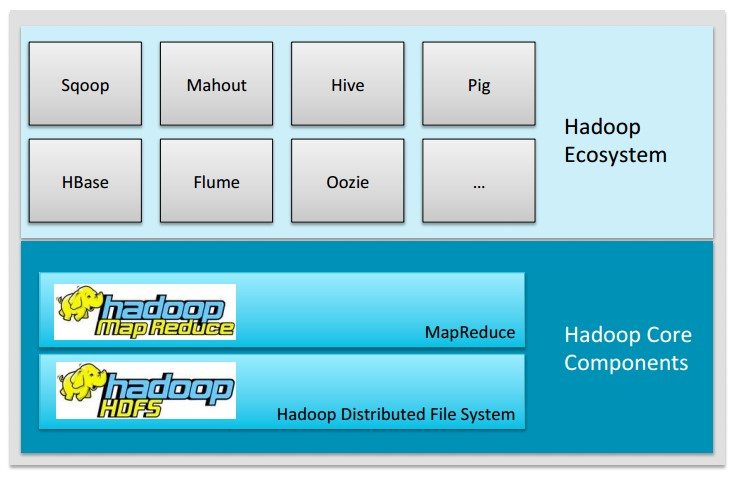
\includegraphics[width=0.9\linewidth]{Chapter4/Chapter4Figs/hadoop}
	\caption{Kiến trúc và hệ sinh thái của Apache Hadoop}
	\label{fig:hadoop}
\end{figure}

Matei Zaharia, cha đẻ của Spark, sử dụng Hadoop từ những ngày đầu. Đến năm $2009$ ông viết Apache Spark\footnote{http://spark.apache.org/} để giải quyết những bài toán học máy ở đại học UC Berkely vì Hadoop MapReduce hoạt động không hiệu quả cho những bài toán này. Rất sớm sau đó ông nhận ra rằng Spark không chỉ hữu ích cho học máy mà còn cho cả việc xử lý luồng dữ liệu hoàn chỉnh. Spark cho phép thực hiện tính toán cùng lúc trên toàn bộ tập dữ liệu mà không cần phải trích xuất mẫu tính toán thử nghiệm. Tốc độ xử lý của Spark có được do việc tính toán được thực hiện cùng lúc trên nhiều máy khác nhau. Đồng thời việc tính toán được thực hiện ở bộ nhớ trong (in-memories) hay thực hiện hoàn toàn trên RAM.

Khi ta có một tác vụ nào đó qúa lớn mà không thể xử lý trên một máy tính/ server, Spark cho phép ta phân chia tác vụ này thành những phần dễ quản lý hơn. Sau đó, Spark sẽ chạy các tác vụ này trong bộ nhớ trên các cluster của nhiều máy tính/server khác nhau để khai thác tốc độ truy xuất nhanh từ RAM. Spark sử dụng API Resilient Distributed Dataset (RDD) để xử lý dữ liệu. Spark nhanh hơn khá nhiều so với cách tiếp cận MapReduce truyền thống.Theo như giới thiệu từ trang chủ của Apache Spark, thì tốc độ của nó nhanh hơn $100x$ so với Hadoop MapReduce khi chạy trên bộ nhớ, và nhanh hơn $10x$ lần khi chạy trên đĩa, tương thích hầu hết các CSDL phân tán (HDFS, HBase, Cassandra, ...). Ta có thể sử dụng Java, Scala, Python hoặc R để triển khai các ứng dụng trên Spark.
\begin{figure}[H]
	\centering
	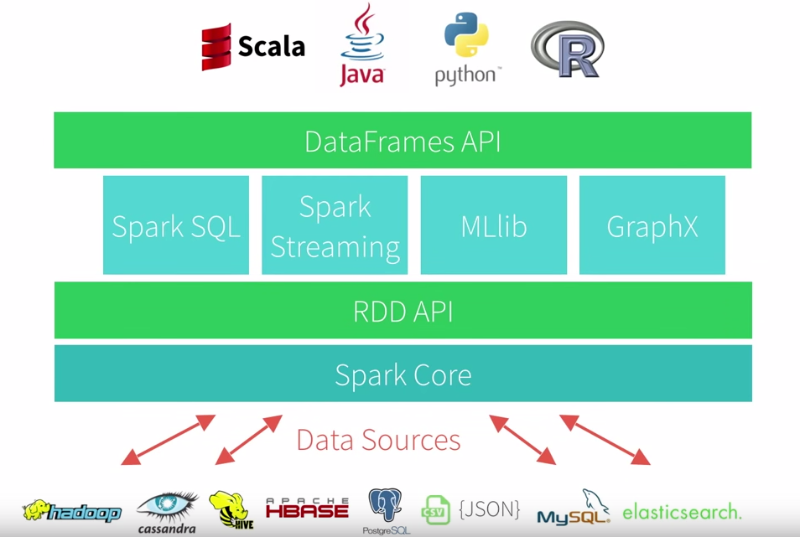
\includegraphics[width=0.9\linewidth]{Chapter4/Chapter4Figs/sparkecosystems}
	\caption{Kiến trúc và hệ sinh thái Apache Spark}
	\label{fig:spark}
\end{figure}

Kiến trúc và hệ sinh thái của Apache gồm:
\begin{itemize}
	\item \textbf{Spark Core:} cung cấp những chức năng cơ bản nhất của Spark như lập lịch cho các tác vụ, quản lý bộ nhớ, fault recovery, tương tác với các hệ thống lưu trữ\dots Đặc biệt, Spark Core cung cấp API để định nghĩa RDD (Resilient Distributed DataSet) là tập hợp của các item được phân tán trên các node của cluster và có thể được xử lý song song.
	\item \textbf{Spark SQL} cho phép truy vấn dữ liệu cấu trúc qua các câu lệnh SQL. Spark SQL có thể thao tác với nhiều nguồn dữ liệu như Hive tables, Parquet, và JSON;
	\item \textbf{Spark Streaming} cung cấp API để dễ dàng xử lý dữ liệu stream;
	\item \textbf{MLlib} Cung cấp rất nhiều thuật toán của học máy như: classification, regression, clustering, collaborative filtering\dots
	\item \textbf{GraphX} là thư viện để xử lý đồ thị.
\end{itemize}
Spark có thể chạy trên nhiều loại Cluster Managers như Hadoop YARN, Apache Mesos hoặc trên chính cluster manager được cung cấp bởi Spark được gọi là Standalone Scheduler.

Một trong những lý do khiến Spark chạy nhanh hơn Hadoop MapReduce đó là ở mỗi tác vụ dữ liệu được nạp lên bộ nhớ và xử lý ở đó, những tác vụ sau có thể sử dụng dữ liệu nằm trên bộ nhớ thay vì phải đọc ghi liên tục vào HDFS như Hadoop MapReduce. Theo một so sánh, năm $2013$ Hadoop sử dụng cluster bao gồm $2100$ máy và mất $72$ phút để sắp xếp $100 TB$ dữ liệu, trong khi Spark cần số lượng máy bằng $1/10$ nhưng sắp xếp chỉ mất $23$ phút. Trong nhiều trường hợp Spark có thể chạy nhanh hơn từ $30-50$ lần so với Hadoop MapReduce.

\begin{figure}[H]
	\centering
	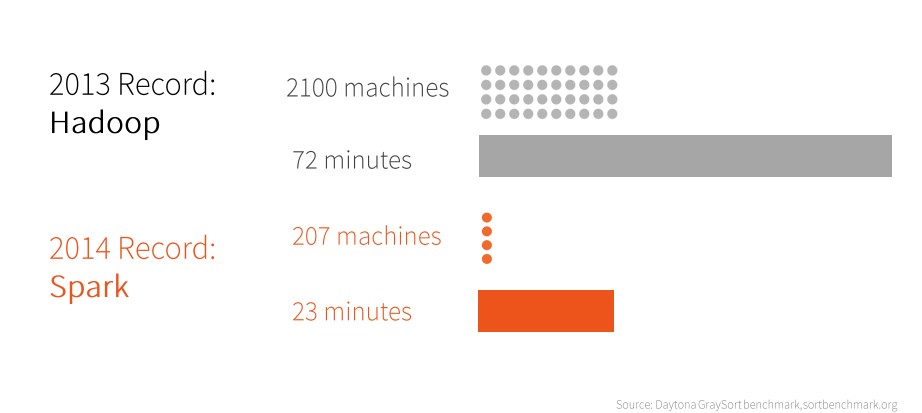
\includegraphics[width=0.9\linewidth]{Chapter4/Chapter4Figs/stark5}
	\caption{So sánh tốc độ sắp xếp $1TB$ dữ liệu của Apache Hadoop và Apache Spark}
	\label{fig:stark5}
\end{figure}

Năm $2015$, Spark trở thành dự án mã nguồn mở sôi động nhất trong lĩnh vực dữ liệu lớn khi thường xuyên được cập nhật bởi hơn $800$ lập trình viên từ $200$ công ty trên khắp thế giới.
\begin{figure}[H]
	\centering
	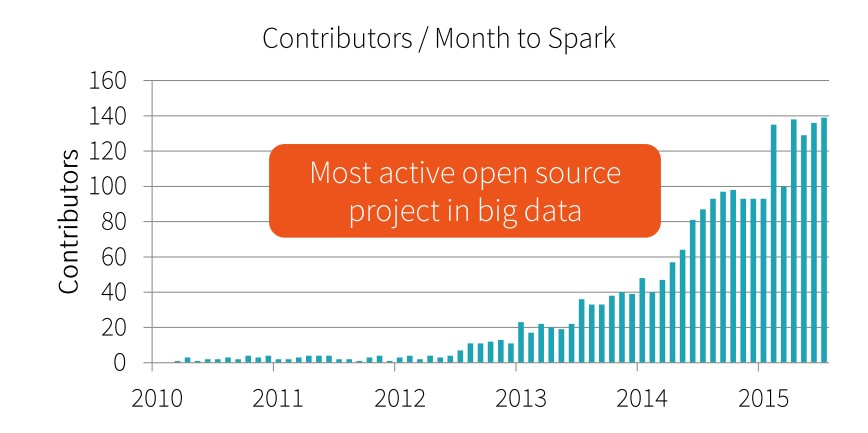
\includegraphics[width=0.9\linewidth]{Chapter4/Chapter4Figs/stark8}
	\caption{Biểu đồ thể hiện sự quan tâm của cộng đồng đến Apache Spark}
	\label{fig:stark8}
\end{figure}


Hình \ref{fig:databricks_2016_spark_survey1} cho thấy các ngôn ngữ và hệ sinh thái của spark được sử dụng trong lập trình các ứng dụng. Dễ thấy Scala và Python là hai ngôn ngữ được sử dụng nhiều nhất trên $58\%$. Các thành phần trong hệ sinh thái được sử dụng khá đồng đều, được sử dụng nhiều nhất là Dataframes và Spark SQL.
\begin{figure}[H]
	\centering
	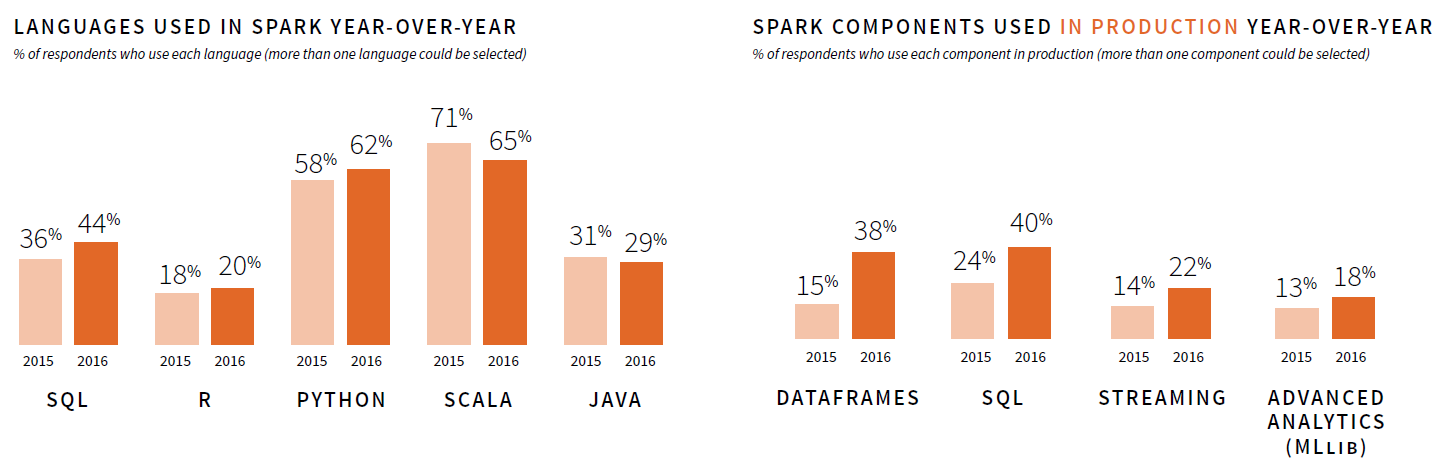
\includegraphics[width=\linewidth]{Chapter4/Chapter4Figs/databricks_2016_spark_survey1.PNG}
	\caption{Biểu đồ thể hiện sự so sánh mức độ quan tâm của các hệ sinh thái Apache Spark}
	\label{fig:databricks_2016_spark_survey1}
\end{figure}

Trong phần phụ lục A đã trình bày chi tiết cách cài đặt và bảng danh sách các lệnh cơ bản khi làm việc trên hai Apache Hadoop \& Spark.

Đề tài này sử dụng hệ sinh thái Apache Spark cho bài toán phát hiện cộng đồng trong mạng có kích thước lớn được lưu trữ phân tán trên HDFS của Hadoop như hình \ref{fig:forrester_spark}. Cụ thể hơn bài toán sử dụng ngôn ngữ Scala do Apache Spark được xây dựng chủ yếu trên Scala vậy nên có tốc độ và hỗ trợ tốt nhất. Ngoài ra do là bài toán xử lý đồ thị lớn nên Graphx là một lựa chọn tốt.
\begin{figure}[H]
	\centering
	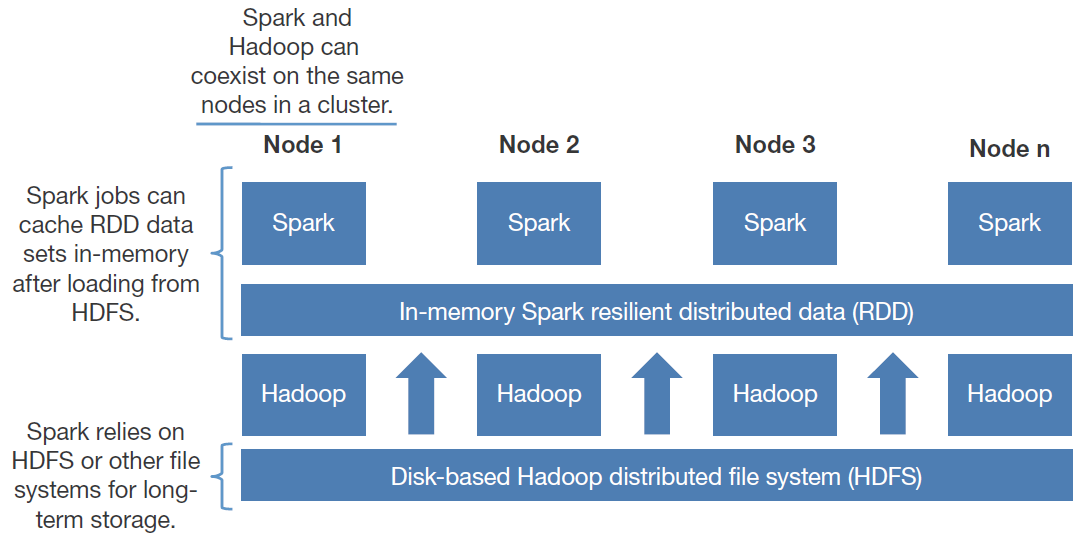
\includegraphics[width=\linewidth]{Chapter4/Chapter4Figs/forrester_spark.PNG}
	\caption{Mô hình kết hợp }
	\label{fig:forrester_spark}
\end{figure}
\subsection{Tính toán song song và phân tán với RDD}
RDD là từ viết tắt của Resilient Distributed Datasets là một cấu trúc dữ liệu cơ bản của Spark. RDD là một tập hợp bất biến phân tán của một đối tượng. Mỗi dataset trong RDD được chia ra thành nhiều phân vùng logical. Có thể được tính toán trên các node khác nhau của một cụm máy tính (cluster). RDDs API hỗ trợ các ngôn ngữ lập trình như Python, Java, Scala, R trong quá trình phát triển ứng dụng. 

Thông thường, RDD chỉ cho phép đọc, phân mục tập hợp của các bản ghi. RDDs có thể được tạo ra trong quá trình xử lý dữ liệu phân tán, RDD là một tập hợp có khả năng chịu lỗi mỗi thành phần có thể được tính toán song song.

Về cơ bản RDD hỗ trợ hai kiểu thao tác thao tác chính:
\begin{itemize}
	\item \textbf{Transformation}: Qua một phương thức transformations thì sẽ cho phép tạo mới một RDD từ RDD đã tồn tại.	Tất cả các transformation đều là lazy, có nghĩa là các transformation này sẽ không thực hiện tính toán ngay mà chúng sẽ được lưu lại thành thành các tập lệnh chờ. Quá trình này có thể hiểu như quá trình lập kết hoạch cho một công việc. Nhờ thiết kế này mà Spark chạy hiệu quả hơn.
	\item \textbf{Action}: Sẽ thực hiện lần lượt các thao tác transformations liên quan đến hành động action đã được lên lịch trước và trả về một và một tập giá trị cho chương trình điều khiển.
\end{itemize}

Bảng \ref{transformation} và \ref{action} giới thiệu các thao tác cơ bản thường được sử dụng trong quá lập trình phân tán song song.
\begin{table}[H]
	\centering
	\caption{Danh sách các thao tác transformation}
	\label{transformation}
	\begin{tabular}{p{1cm}p{5cm}p{10cm}}
		\toprule
		\textbf{STT} & \multicolumn{1}{c}{Thao tác}                        & \multicolumn{1}{c}{\textbf{Ý nghĩa}}                                                                                                                                                                                                       \\ \midrule
		1            & \textbf{map(func)}                                  & Trả về 1 RDD mới bằng cách truyền mỗi phần tử đầu vào qua hàm func.                                                                                                                                                                        \\ \midrule
		2            & \textbf{filter(func)}                               & Trả về 1 RDD mới bằng cách chọn những phần tử đầu vào(nguồn) mà hàm func,trả về kết quả true.                                                                                                                                              \\ \midrule
		3            & \textbf{flatMap(func)}                              & Tương tự map nhưng khác map ở chỗ, mỗi phần tử đầu vào quaflatMap sẽ trả về 0 hoặc nhiều phần tử đầu ra(có thể hiểu quamap sẽ là 1-1).                                                                                                     \\ \midrule
		4            & \textbf{mapPartitions(func)}                        & Tương tự như map,nhưng chạy riêng biệt trên mỗi vùng RDD,Hàmfunc, phải có dạng Iterator{[}T{]} =\textgreater  terator{[}U{]} khi chạy RDD kiểuT.                                                                                           \\ \midrule
		5            & \textbf{union(otherDataset)}                        & Trả về 1 RDD mới là hợp của tập dữ liệu phần tử đầu vào(nguồn) và các phần tử của đối(otherDataset).                                                                                                                                       \\ \midrule
		6            & \textbf{distinct({[}numTasks{]}))}                  & Trả về 1 RDD mới chứa mỗi phần tử là duy nhất của tập dữ liệunguồn.                                                                                                                                                                        \\ \midrule
		7            & \textbf{groupByKey({[}numTasks{]})}                 & Khi gọi đến 1 tập dữ liệu (K,V) sẽ trả về 1 tập là cặp (K,Seq(V))( Tức là nhóm tập các phần tử cùng Key). Chú ý: mặc định chỉ có 8 task song song khi grouping. Có thể thay đổi số task song song này bằng việc truyềnvào tham số đầu vào. \\ \midrule
		8            & \textbf{reduceByKey(func, {[}numTasks{]})}          & Khi gọi tập dữ liệu (K,V), trả về 1 tập (K,V) mà giá trị của key đượctổng hợp sử dụng hàm reduce func.                                                                                                                                     \\ \midrule
		9            & \textbf{sortByKey({[}ascending{]}, {[}numTasks{]})} & Khi gọi tập dữ liệu (K,V) với K có thể thực hiện sắp thứ tự được.Khi đó, nó sẽ trả về tập dữ liệu (K,V) được sắp sếp tăng dần hoặcgiảm dần theo key. Chú ý: ascending là kiểu Boolean.                                                     \\ \midrule
		10           & \textbf{join(otherDataset, {[}numTasks{]})}         & Khi gọi tập dữ liệu có kiểu (K,V) và (K,W), nó sẽ trả về 1 cặp mới(K,(V,W)) ( nối 2 phần tử có cùng key).                                                                                                                                  \\ \midrule
		11           & \textbf{cogroup(otherDataset, {[}numTasks{]})}      & Khi gọi tập dữ liệu có kiểu (K,V) và (K,W), nó sẽ trả về 1 tập dữ liệu (K,seq(V),seq(W)).                                                                                                                                                  \\ \midrule
		12           & \textbf{cartesian(otherDataset)}                    & Khi gọi 1 tập dữ liệu kiểu T và U, nó sẽ trả về tập dữ liệu mới (T,U).                                                                                                                                                                     \\ \bottomrule
	\end{tabular}
\end{table}

\begin{table}[H]
	\centering
	\caption{Danh sách các thao tác action}
	\label{action}
	\begin{tabular}{p{1cm}p{5cm}p{10cm}}
		\toprule
		\textbf{STT} & \multicolumn{1}{c}{Thao tác}  & \multicolumn{1}{c}{\textbf{Ý nghĩa}}                                                                                                                   \\ \midrule
		1            & \textbf{reduce(func)}         & Tổng hợp các phần tử của tập dữ liệu sử dụng hàm func(có 2 đối vàtrả về 1 kết quả).                                                                    \\ \midrule
		2            & \textbf{collect()}            & Trả về tất cả các phần tử của tập dữ liệu như 1 mảng ở driverProgram. Hàm này hữu ích sau khi lọc hoặc thao tác khác màtrả về tập dữ liệu con đủ nhỏ.  \\ \midrule
		3            & \textbf{count()}              & Trả về số phần tử của tập dữ liệu                                                                                                                      \\ \midrule
		4            & \textbf{first()}              & Trả về phần tử đầu tiên của tập dữ liệu( tương tự take(1)).                                                                                            \\ \midrule
		5            & \textbf{take(n)}              & Trả về mảng gồm n phần tử đầu tiên của tập dữ liệu.                                                                                                    \\ \midrule
		6            & \textbf{saveAsTextFile(path)} & Ghi các phần tử của tập dữ liệu như 1 file text( hoặc tập file text)lên 1 thư mục trong hệ thống local, HDFS hoặc hệ thống hỗ trợ Hadoop bất kỳ.       \\ \midrule
		7            & \textbf{countByKey()}         & Chỉ cho RDD có kiểu (K,V). Trả về 1 Map (K,Int). Int là chỉ số key.                                                                                    \\ \midrule
		8            & \textbf{foreach(func)}        & Chạy hàm func cho mỗi phần tử của tập dữ liệu. Điều này có tác dụngkhi thực hiện cập nhật 1 biến accumulator hoặc tương tác vớihệ thống lưu trữ ngoài. \\ \bottomrule
	\end{tabular}
\end{table}
%\subsection{GraphX}
%GraphX là một phần trong hệ sinh thái của Apache Spark hay có thể nói là một thư viện hỗ trợ tổ chức dữ liệu đồ thị dưới dạng phân tán trên nhiều máy trong cụm và các thuật toán hỗ trợ xử lý đồ thị. Nhờ vậy GraphX rất vượt trội và phù hợp trong bài toán xử lý đồ thị có kích thước lớn đặc biệt với bài toán của khóa luận này.
\section{Thực nghiệm}
Để kiểm chứng phương pháp phát hiện cộng đồng sử dụng mô hình BigCLAM, phương pháp đã được tiến hành cài đặt thực nghiệm trên môi trường cụm máy tính có cấu hình như bảng \ref{hatangtinhtoan} sử dụng Apache Hadoop trong việc lưu trữ phân tán và Apache Spark trong tính toán phân tán. Trong quá trình thực nghiệm, có sử dụng một vài cấu trúc mạng có kích thước tương đối lớn như trong bảng \ref{testgraphformethod}.
\begin{table}[H]
	\centering
	\caption{Thông số hệ thống sử dụng trong thực nghiệm}
	\label{hatangtinhtoan}
	\begin{tabular}{@{}clcc@{}}
		\toprule
		\multicolumn{1}{l}{STT} & Thông số                                                                                                                              & \multicolumn{1}{l}{Số lượng} & \multicolumn{1}{l}{Vai trò} \\ \midrule
		$1$                     & \begin{tabular}[c]{@{}l@{}}OS: Ubuntu $16.04$ LTS\\ HDD: $95$ GB\\ RAM: $4$ GB\\ CPU: intel Core i5-4590U CPU $3.30GHz$ x $4$\end{tabular} & $1$                            & master                      \\ \midrule
		$2$                     & \begin{tabular}[c]{@{}l@{}}OS: Ubuntu $16.04$ LTS\\ HDD: $95$ GB\\ RAM: $4$ GB\\ CPU: intel Core i5-4590U CPU $3.30GHz$ x $4$\end{tabular} & $9$                           & workers                     \\ \bottomrule
	\end{tabular}
\end{table}
Trong quá trình thực nghiệm tôi đã sử dụng sử dụng các thao tác với RDDs như trong bảng \ref{transformation} và \ref{action} để thực hiện tính toán phân tán. 
\begin{table}[H]
	\centering
	\caption{Mô tả các mạng sử dụng để thực nghiệm}
	\label{testgraphformethod}
	\begin{tabular}{@{}lrr@{}}
		\toprule
		Tên mạng                & Số đỉnh      & Số cạnh         \\ \midrule
		Mạng xã hội facebook & $4,039$  & $88,234$        \\
		Mạng cộng tác ca-HepTh      & $9,877$    & $25,998$    \\
		Mạng cộng tác ca-AstroPh     & $18,772$  & $198,110$     \\
		Mạng small internet  & $22,963$ & $48,436$    \\
		Mạng Email-Enron      & $36,692$  & $367,662$    \\
		
		 \bottomrule
	\end{tabular}
\end{table}
\begin{figure}[H]
	\label{bd:thucnghiem}
	\centering
\begin{tikzpicture}
\begin{axis}[title  = Biểu đồ thể hiện thời gian chạy và số lượng cộng đồng phát hiện được trên mỗi mạng,
xbar,
height=10cm,
width=15cm,
y axis line style = { opacity = 0 },
axis x line       = none,
tickwidth         = 0pt,
enlarge y limits  = 0.2,
enlarge x limits  = 0.02,
symbolic y coords = {Email-Enron,Internet,AstroPh,CA-HepTH,Facebook},
nodes near coords,
]
\addplot coordinates { (1.5,Facebook)         (13.2,Internet)
	(18.8,AstroPh)  (3.8,CA-HepTH) (20.9,Email-Enron)  };
\addplot coordinates { (120,Facebook)         (450,Internet)
	(720,AstroPh)   (250,CA-HepTH) (590,Email-Enron) };
\legend{Thời gian chạy (phút), Số cộng đồng}
\end{axis}
\end{tikzpicture}
\caption{Kết quả thực nghiệm}
\end{figure}
Hình 4.7 chính là kết quả quá trình thực nghiệm của các mạng trong bảng \ref{testgraphformethod}. Có thể thấy thời gian thực nghiệm trên khá tốt. Và hình \ref{fig:facebook-demo} và \ref{fig:graph3} là kết quả của việc mô phỏng phân bố của các cộng đồng trong mạng xã hội facebook và Internet trong bảng \ref{testgraphformethod}.
\begin{figure}[]
	\centering
	\begin{minipage}[t]{0.48\textwidth}
		\centering
		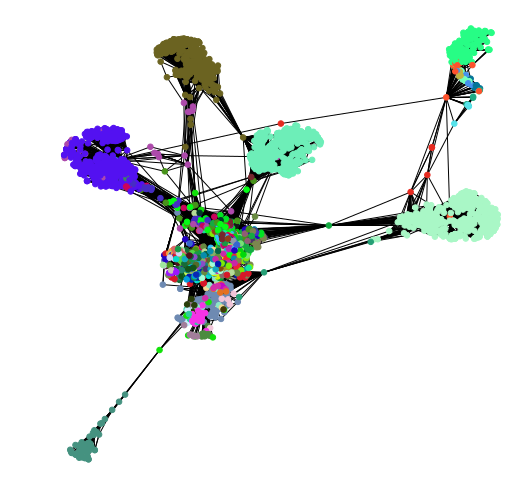
\includegraphics[width=\linewidth]{Chapter3/Chapter3Figs/facebook_demo}
		\caption{Mô phỏng phát hiện cồng đồng trên mạng facebook \ref{testgraphformethod}}
		\label{fig:facebook-demo}
	\end{minipage}
	\begin{minipage}[t]{0.48\textwidth}
		\centering
		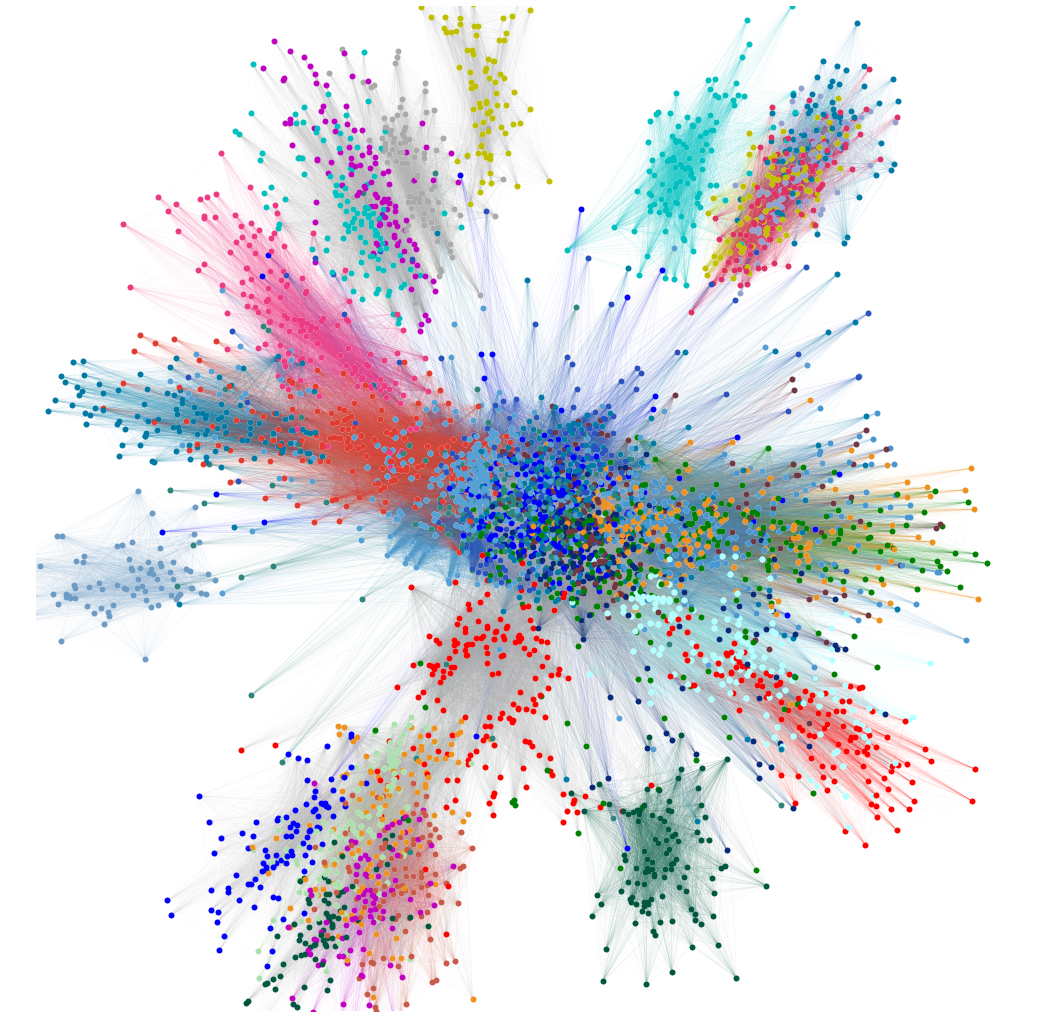
\includegraphics[width=0.7\linewidth]{Chapter3/Chapter3Figs/graph}
		\caption{Mô phỏng phát hiện cồng đồng trên mạng internet \ref{testgraphformethod}}
		\label{fig:graph3}
	\end{minipage}    
\end{figure}

Ngoài ra, việc sử dụng một vài khái niệm sau đã cải thiện hiệu năng đáng kể:
\begin{itemize}
	\item Biến broadcast: được tạo ra bằng cách gọi hàm SparkContext.broadcast(v). Broadcast variable là một wrapper xung quanh biến v, giá trị của biến này có thể được truy xuất thông qua hàm value. Về cơ bản biến broadcast sẽ được phân tán biến biến local trên tất cả các máy worker, điều này làm giảm thời gian cho các máy worker quay trở lại máy master để lấy giá trị.
	\item Biến accumulator: Khi ta muốn thực hiện các thao tác trên tập dữ liệu được phân tán mà không thể thông qua các thao tác RDD hỗ trợ thì biến accumulator cho phép là một biến trung gian (toàn cục) giữa các máy trong cụm. 
	\item phương thức cache/ persist: Cho phép dữ liệu được lưu trữ trên RAM. Điều này giúp cho các tác vụ được sử dụng nhiều lần sẽ có thời gian truy vấn nhanh hơn do dữ liệu đã lưu lại trên RAM.
\end{itemize}

Để quá trình huấn luyện theo công thức \ref{eq:ctfu_hat} trên hệ thống phân phán phát huy tính hiệu quả. Tôi đã đề xuất sử dụng phương pháp tăng gradient ngẫu nhiên theo cụm đã được trình bày trong thuật toán \ref{alg:MBSGD}.